\documentclass[aspectratio=43]{beamer}
\usetheme{CCNU}
%\usefonttheme[onlymath]{serif}

\usepackage{slashed}
\usepackage{datetime}
%\usepackage{slidesphysics}
\graphicspath{{../img/}}
\usepackage{hyperref}
\usepackage{cancel}
% \hypersetup{colorlinks=true, 
%     linkcolor=blue,          % color of internal links (change box color with linkbordercolor)
%     citecolor=black,        % color of links to bibliography
%     filecolor=black,      % color of file links
%     urlcolor=blue    }
% \usepackage{deflamb}
% \usepackage{color, colortbl}
% \usepackage{tikz}
%\usepackage{userdef}
\usepackage[absolute,overlay]{textpos}
\def\Put(#1,#2)#3{\leavevmode\makebox(0,0){\put(#1,#2){#3}}}

\def\mydate{\leavevmode\hbox{\the\year-\twodigits\month-\twodigits\day}}
\def\twodigits#1{\ifnum#1<10 0\fi\the#1}

\newcommand\Wider[2][3em]{%
\makebox[\linewidth][c]{%
  \begin{minipage}{\dimexpr\textwidth+#1\relax}
  \raggedright
  \centering#2
  \end{minipage}%
  }%
}

%\def\meetingname{Alicia Garrido Peña. PhD thesis Presentation}


\def\meetingname{Alicia Garrido Peña. PhD thesis Seminar}

\title[\meetingname]{Characterization of the sequential nature of neuronal dynamics: Experimental recordings, computational models and novel stimulation neurotechnologies}
\author[A. Garrido-Peña]{Alicia Garrido Peña}
% \institute[Michigan]{}
\institute[UAM]{Universidad Autónoma de Madrid}
\date[\mydate]{\meetingname\\\today}

\begin{document}
\begin{frame}[plain,t]
\titlepage
\end{frame}

%The next statement creates the title page.
\begin{frame}
\frametitle{Contents}
\tableofcontents
\end{frame}
%------------------------------------------------------------
\section{Introduction}
\begin{frame}{Neuroscience}
	\only<1>{\includegraphics[width=\textwidth]{intro/neurosciences.pdf}}
	\only<2>{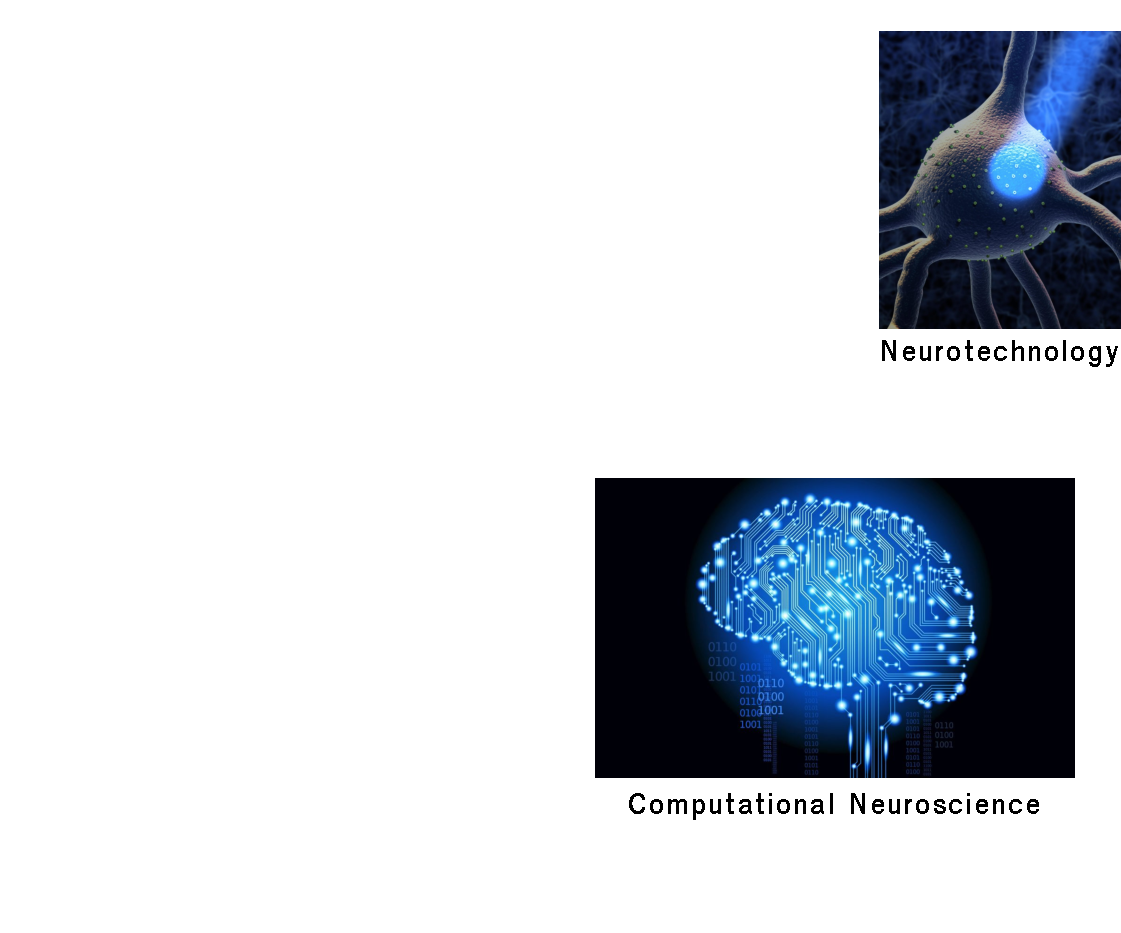
\includegraphics[width=\textwidth]{intro/neurosciences_focus.pdf}}
\end{frame}
\begin{frame}{Approach}
	\begin{itemize}
		\item Neurocomputational Perspective
		\item<2-> Bottom-up approach
		\item<5-> Combining electrophysiology \uncover<6>{and computational work}
	\end{itemize}
	\vfill
	\centering
	\uncover<3-4>{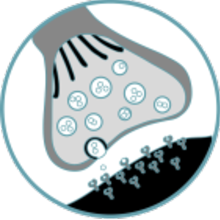
\includegraphics[width=0.3\textwidth]{intro/ions.pdf}}
	\hspace{30pt}
	\uncover<4-4>{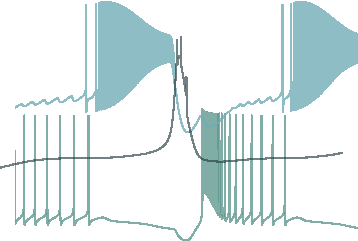
\includegraphics[width=0.4\textwidth]{intro/CPG.pdf}}
	\uncover<3-4>{\\From ionic channels}
	\uncover<4-4>{\hspace{50pt} To minimal circuits}
\end{frame}

\begin{frame}{Neuronal and Networks Dynamics}
	\only<1>{Neuronal electrical activity is often described in terms of the evolution of membrane voltage caused by the flow of ionic channels between the inside and outside of the cell.}
	
	\uncover<2->{Depending on the channels that constitute the neuron and the circuit it is immersed in, the activity varies.}
	\vfill
	\uncover<3->{In terms of the spike waveform:}
	\uncover<3->{\begin{center}
			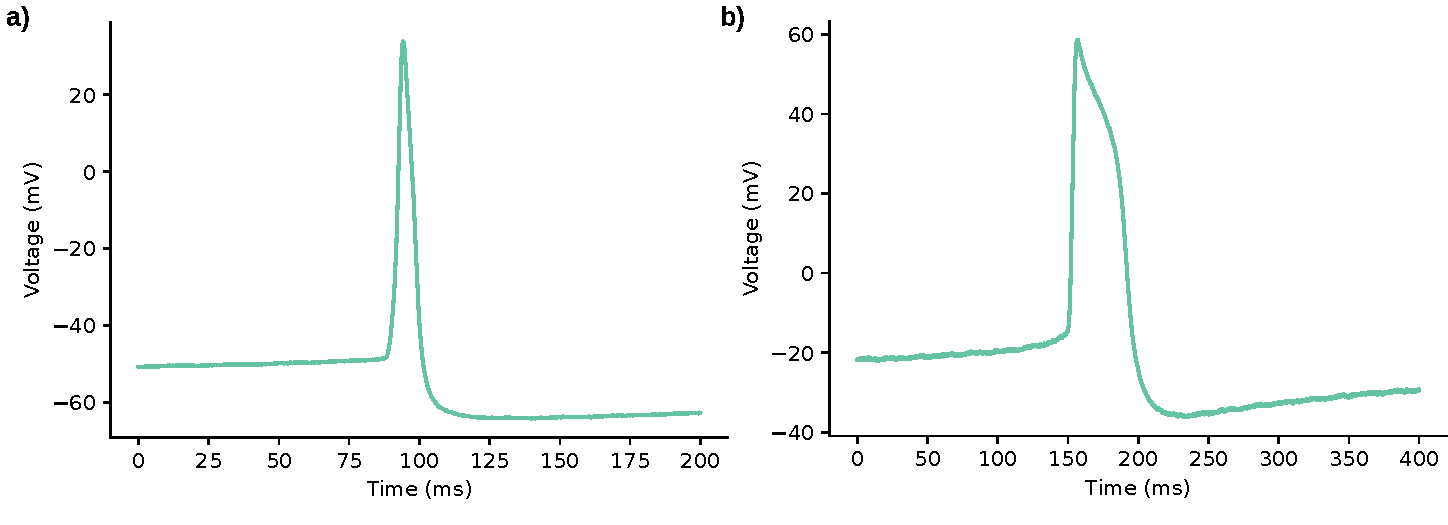
\includegraphics[width=0.7\textwidth]{intro/spike-types.pdf}
	\end{center}}
	
	\uncover<4->{\vfill}
	\uncover<4->{And the type of spiking activity: tonic firing, bursting, etc.}
	\uncover<4->{\begin{center}
			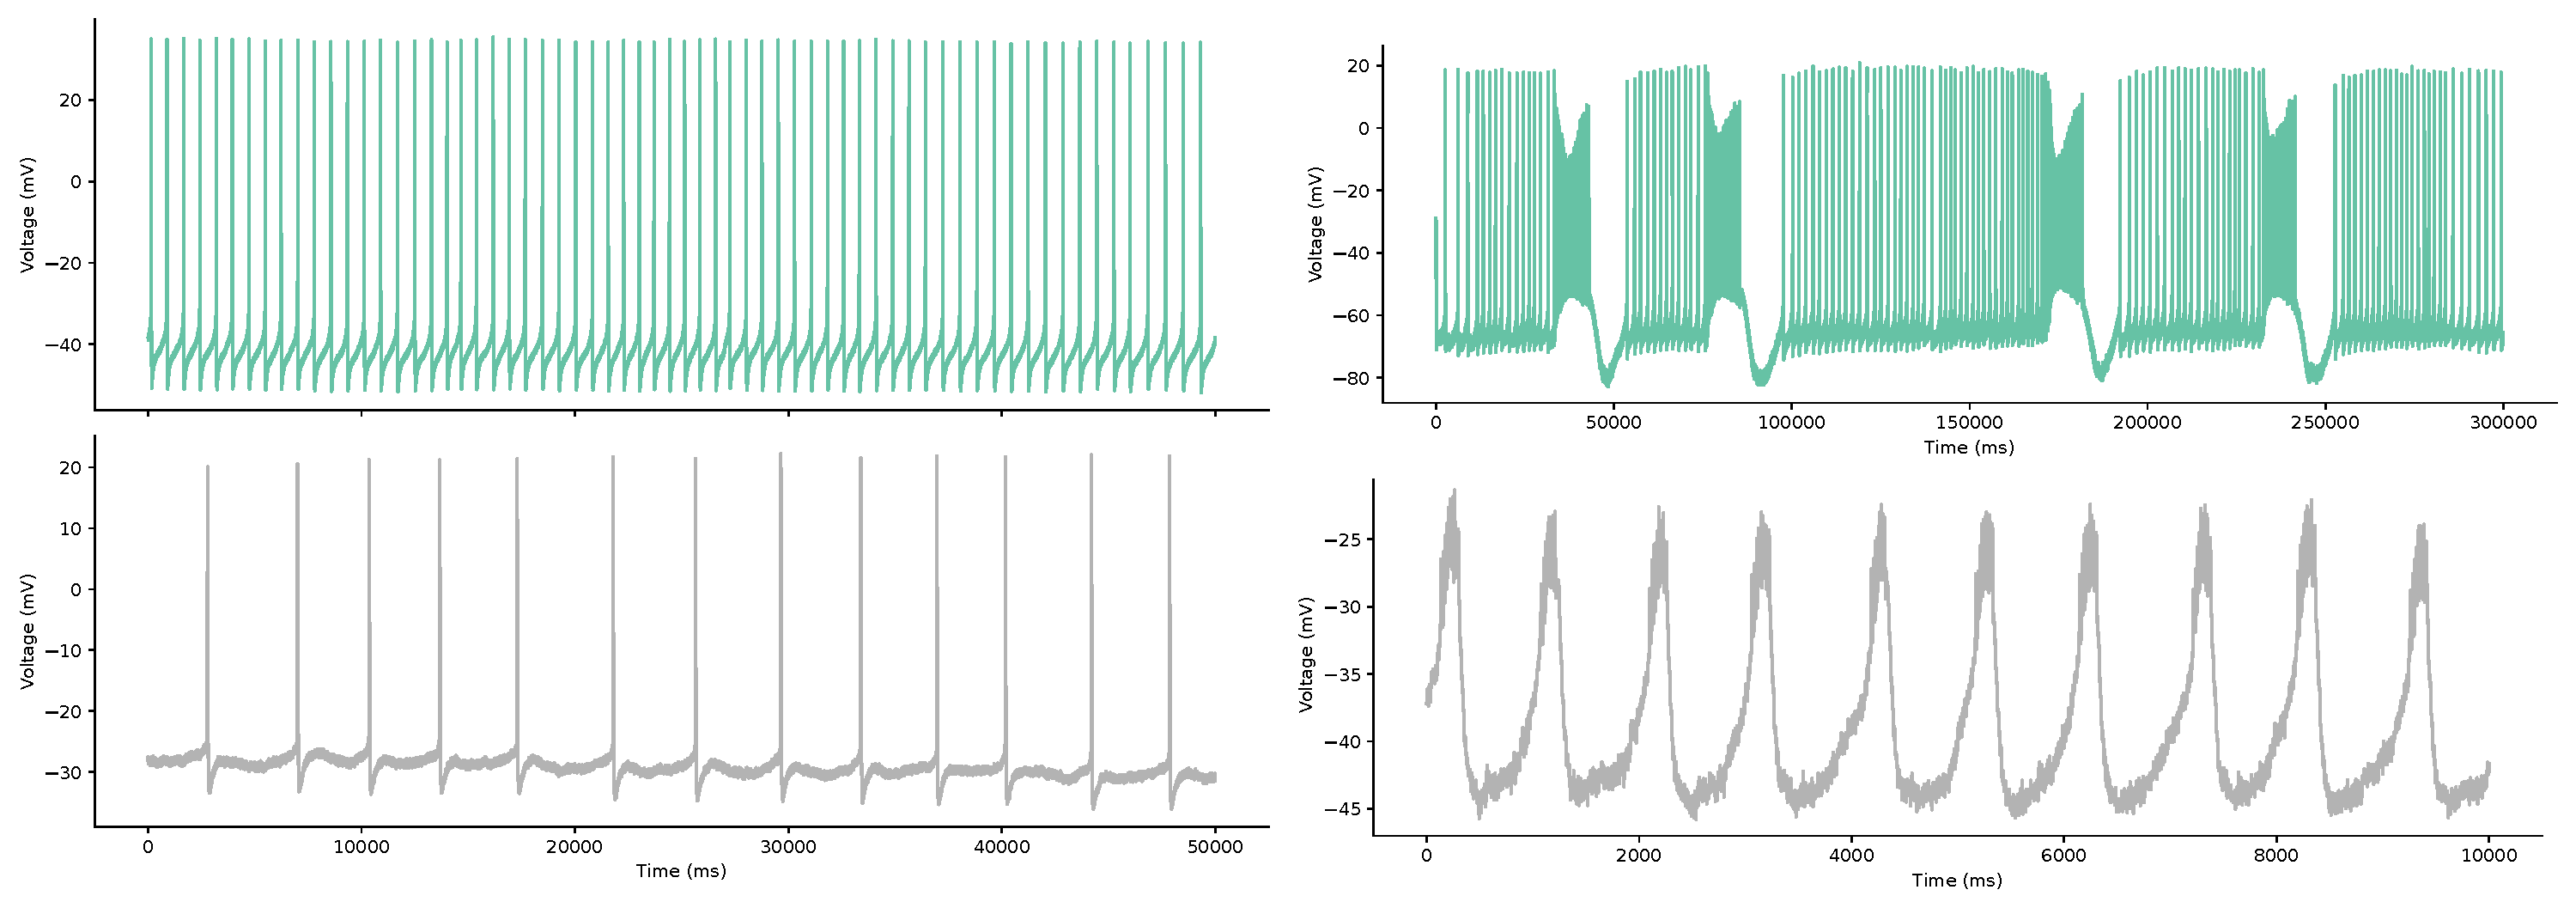
\includegraphics[width=0.7\textwidth]{intro/spike_activity-types.pdf}
	\end{center}}
\end{frame}

\begin{frame}{The sequential nature of neural dynamics}
	 \begin{columns}
			\begin{column}{0.6\textwidth}
				\begin{itemize}
					\item<1->{There are sequential processes at different time-scales.} 
					\item<3->{Many behaviors and actions are governed by sequential processes}
					\item<4->{Motor control, speech, decision making, etc. }
%					\item<5->{Studying sequential activity at different scales is crucial for a complete comprehension of neural systems.}
					\item<5->{Sequential dynamical invariants might have a crucial role in neural coordination to autonomously establish a balance between the robustness and flexibility required for effective function.}
				\end{itemize}
			\end{column}
			\begin{column}{0.45\textwidth}
				\uncover<2->{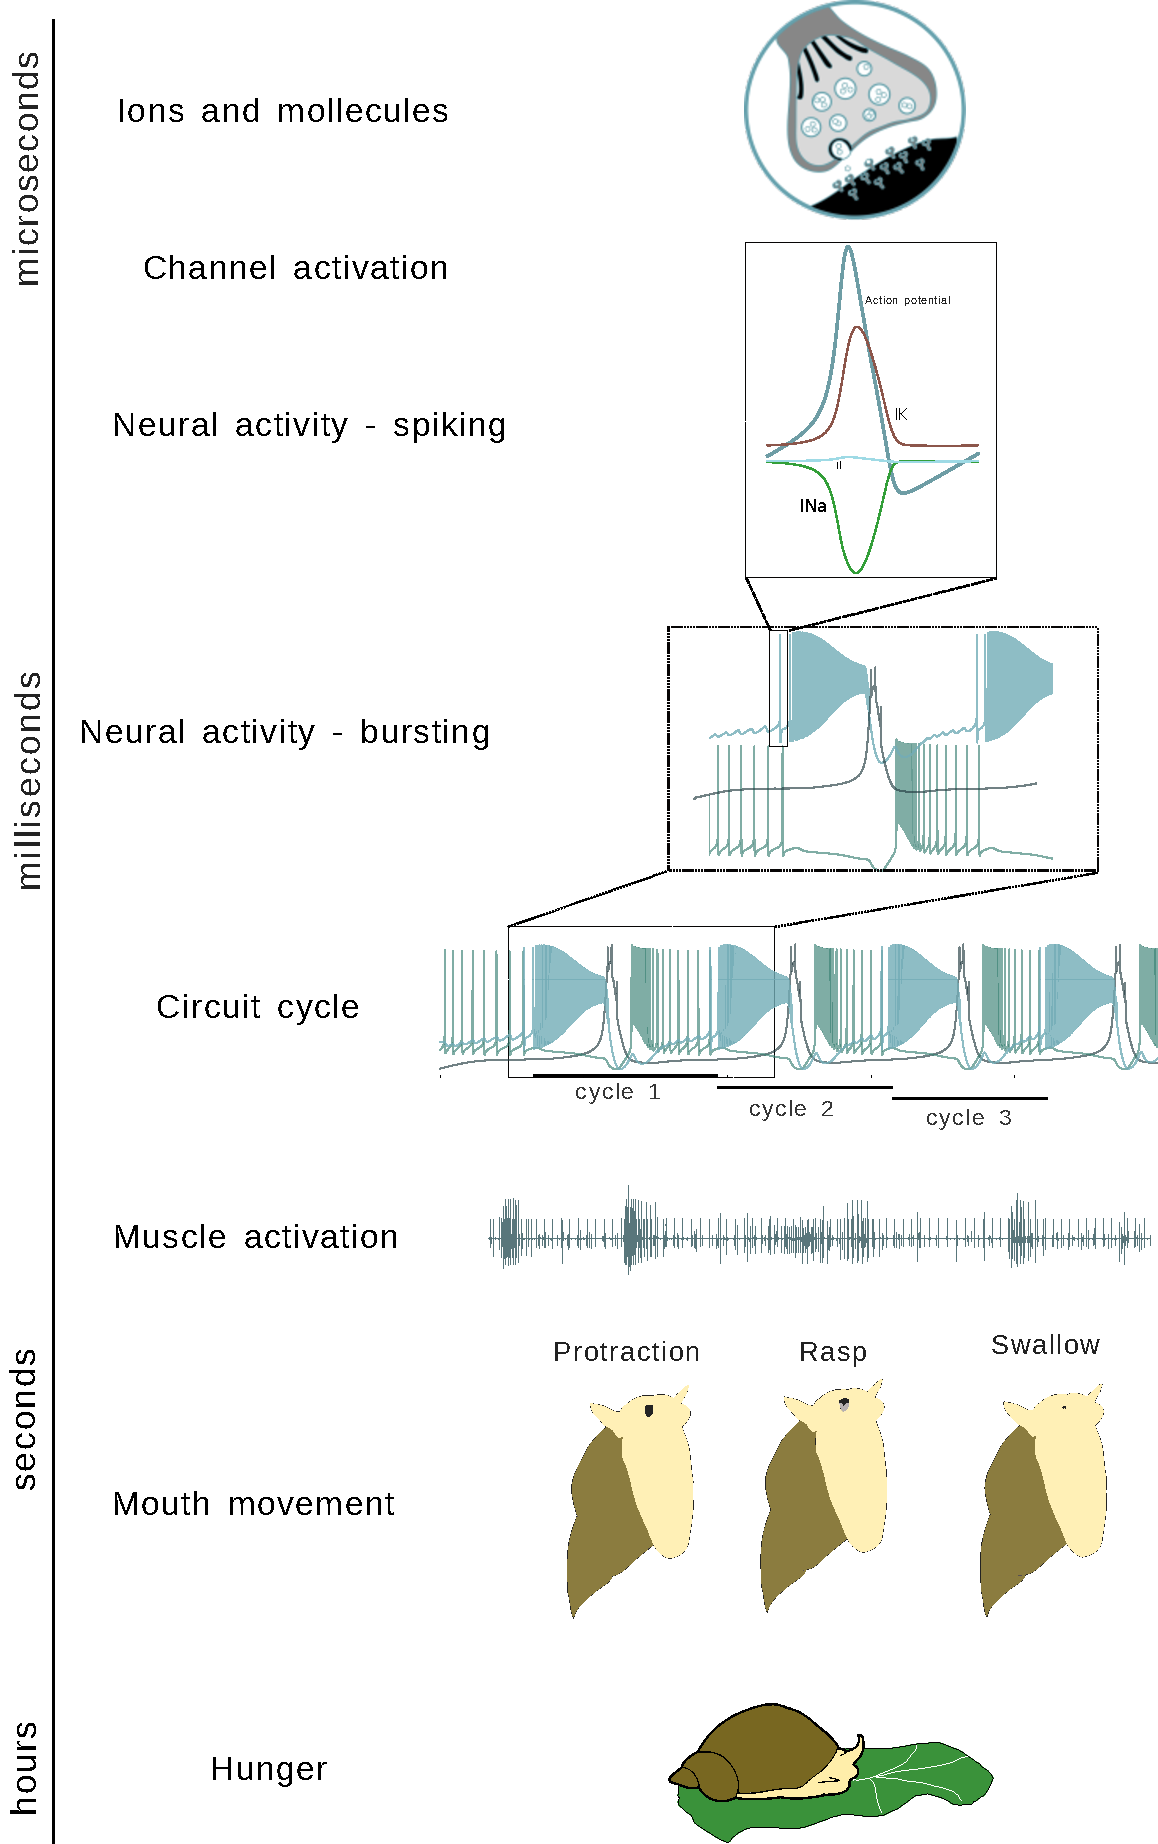
\includegraphics[width=\textwidth]{intro/time scale/time-scale-feeding.pdf}}
			\end{column}
		\end{columns}
	 
\end{frame}

\begin{frame}{Studying neural dynamics in computational models}
	\begin{itemize}
		\item<1-8>{Computational models are powerful tools to study neural dynamics}
		\item<2-8>{Advantages}
		\begin{itemize}
			\item<3-8>Full accessibility to the 
			\item<4-8>Detailed reproduction of the living activity
		\end{itemize}
		\item<5-8>{Limitations}
		\begin{itemize}
			\item<6-8>{Restricted variability}
			\item<7-8>{The description may depend on the information about the living system}
		\end{itemize}
	\end{itemize}
\end{frame}

\begin{frame}{Studying neural dynamics in computational models}
	\uncover<1->{\textbf{Conductace-based models}}
	 \uncover<1-2>{
		\begin{table}[h!]
			\resizebox{\textwidth}{!}{%
				\begin{tabular}{lccc}
					Voltage equation                                                                 & \multicolumn{3}{c}{$C \frac{dV}{dt} = I - g_K n^4 (V - E_K) - g_{Na} m^3h(V-E_{Na}) - g_L (V-E_L)$}                                                                                                                                  \\ \hline
					& \multicolumn{2}{c}{Activation variables}                                                                                                                              & Inactivation variable                                        \\ \hline
					\multicolumn{1}{c|}{\begin{tabular}[c]{@{}c@{}}gating \\ variables\end{tabular}} & \multicolumn{1}{c|}{$\frac{dm(t)}{dt}=\frac{m_{\infty}(V(t))-m(t)}{\tau_m(V(t))}$} & \multicolumn{1}{c|}{$\frac{dn(t)}{dt}=\frac{n_{\infty}(V(t))-n(t)}{\tau_n(V(t))}$} & $\frac{dh(t)}{dt}=\frac{h_{\infty}(V(t))-h(t)}{\tau_h(V(t))}$ \\ \hline
				\end{tabular}%
			}
	\end{table}}

\end{frame}

\begin{frame}{Studying neural dynamics in computational models}
	\uncover<1->{\textbf{Conductace-based models}}	
	\\
	\uncover<3-4>{By different combinations of ionic channels we can achive different activities and waveform shapes}
	\uncover<4>{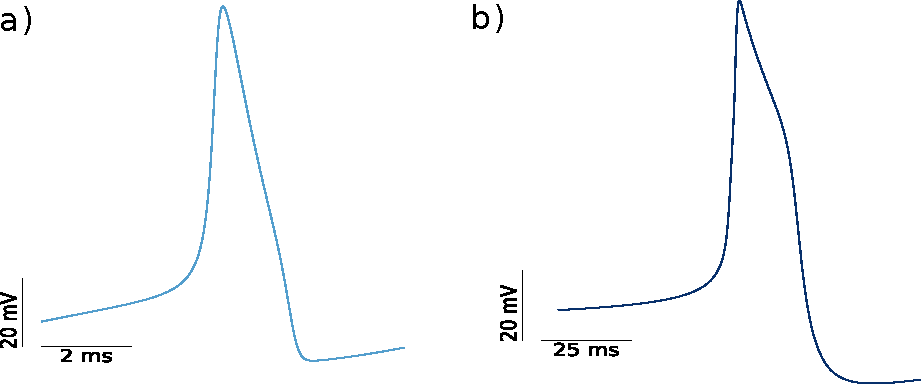
\includegraphics[width=\linewidth]{intro/spike-types model.pdf}}

\end{frame}

\begin{frame}{Studying neural dynamics in computational models}
	\uncover<1->{\textbf{Conductace-based models\\}}
	\only<5-6>{By modeling synapses we can model whole circuits by connecting single modeled neurons.\\}
	\only<6>{\centering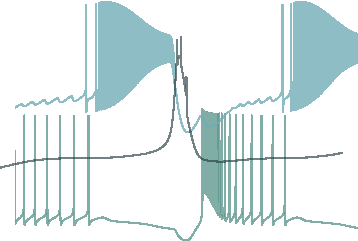
\includegraphics[width=0.7\linewidth]{intro/cpg.pdf}}
\end{frame}


\begin{frame}{Vertebrate and invertebrate animal studies}
\end{frame}
\begin{frame}{Neural stimulation}
	    \end{frame}

\section{Motivation and Objectives}
\begin{frame}{Motivation and Objectives}
\end{frame}

\section{Conclusion}

    \begin{frame}{Conclusion}
    \end{frame}
%}
%\setbeamercolor{background canvas}{bg=violet}
\setbeamercolor{background canvas}{bg=CCNUMaize}
\begin{frame}[plain,t]
\vspace{100pt}
\centering

\includegraphics[width=0.6\textwidth]{logos/UAM+EPS_L-eps-converted-to.pdf}
\end{frame}
\end{document}